%%%%%%%%%%%%%%%%%%%%%%%%%%%%%%%%%%%%%%%%%
% Journal Article
% LaTeX Template
% Version 1.4 (15/5/16)
%
% This template has been downloaded from:
% http://www.LaTeXTemplates.com
%
% Original author:
% Frits Wenneker (http://www.howtotex.com) with extensive modifications by
% Vel (vel@LaTeXTemplates.com)
%
% License:
% CC BY-NC-SA 3.0 (http://creativecommons.org/licenses/by-nc-sa/3.0/)
%
%%%%%%%%%%%%%%%%%%%%%%%%%%%%%%%%%%%%%%%%%
%----------------------------------------------------------------------------------------
%	PACKAGES AND OTHER DOCUMENT CONFIGURATIONS
%----------------------------------------------------------------------------------------

\documentclass[twoside,twocolumn]{article}

\usepackage{blindtext} % Package to generate dummy text throughout this template

\usepackage[sc]{mathpazo} % Use the Palatino font
\usepackage[utf8]{inputenc}
\usepackage[T1]{fontenc} % Use 8-bit encoding that has 256 glyphs
\linespread{1.05} % Line spacing - Palatino needs more space between lines
\usepackage{microtype} % Slightly tweak font spacing for aesthetics

\usepackage[french]{babel} % Language hyphenation and typographical rules

\usepackage[hmarginratio=1:1,top=32mm,columnsep=20pt]{geometry} % Document margins
\usepackage[hang, small,labelfont=bf,up,textfont=it,up]{caption} % Custom captions under/above floats in tables or figures
\usepackage{booktabs} % Horizontal rules in tables

\usepackage{lettrine} % The lettrine is the first enlarged letter at the beginning of the text

\usepackage{enumitem} % Customized lists
\setlist[itemize]{noitemsep} % Make itemize lists more compact

\usepackage{abstract} % Allows abstract customization
\renewcommand{\abstractnamefont}{\normalfont\bfseries} % Set the "Abstract" text to bold
\renewcommand{\abstracttextfont}{\normalfont\small\itshape} % Set the abstract itself to small italic text

\usepackage{titlesec} % Allows customization of titles
\renewcommand\thesection{\Roman{section}} % Roman numerals for the sections
\renewcommand\thesubsection{\roman{subsection}} % roman numerals for subsections
\titleformat{\section}[block]{\large\scshape\centering}{\thesection.}{1em}{} % Change the look of the section titles
\titleformat{\subsection}[block]{\large}{\thesubsection.}{1em}{} % Change the look of the section titles

\usepackage{fancyhdr} % Headers and footers
\pagestyle{fancy} % All pages have headers and footers
\fancyhead{} % Blank out the default header
\fancyfoot{} % Blank out the default footer
\fancyhead[C]{Rapport d'avancement de Thèse $\bullet$ \today} % Custom header text
\fancyfoot[RO,LE]{\thepage} % Custom footer text

\usepackage{titling} % Customizing the title section

\usepackage{hyperref} % For hyperlinks in the PDF

\usepackage{graphicx}

\usepackage{csquotes}
\usepackage[style=ieee,backend=bibtex]{biblatex}

\bibliography{biblio}

%----------------------------------------------------------------------------------------
%	TITLE SECTION
%----------------------------------------------------------------------------------------

\setlength{\droptitle}{-4\baselineskip} % Move the title up

\pretitle{\begin{center}\normalsize Rapport d'avancement \\
\Huge\bfseries} % Article title formatting
\posttitle{\end{center}} % Article title closing formatting
\title{Systèmes Cyber-Physiques autonomes et communicants en milieux hostiles. Application à l’exploration par robots mobiles. } % Article title
\author{%
\textsc{Virgile Daugé} \\[1ex] % Your name
\normalsize L.O.R.I.A. \\ % Your institution
\normalsize \href{mailto:virgile.dauge@inria.fr}{virgile.dauge@inria.fr} % Your email address
%\and % Uncomment if 2 authors are required, duplicate these 4 lines if more
%\textsc{Jane Smith}\thanks{Corresponding author} \\[1ex] % Second author's name
%\normalsize University of Utah \\ % Second author's institution
%\normalsize \href{mailto:jane@smith.com}{jane@smith.com} % Second author's email address
}
\date{\today} % Leave empty to omit a date
\renewcommand{\maketitlehookd}{%

%----------------------------------------------------------------------------------------
%	Abstract
%----------------------------------------------------------------------------------------

\begin{abstract}
\noindent L'objectif de ce rapport est de présenter brièvement l'avancement de mes travaux.
Premièrement, un rapide état de l'art des technologies permettant l'exploration autonome sera dréssé.
Suivie par une analyse des solutions existantes ainsi que les axes de développement dégagés.
Ce document ne représente qu'un bref résumé et n'est donc pas exhaustif.
\end{abstract}
}

%----------------------------------------------------------------------------------------

\begin{document}

% Print the title
\maketitle

%----------------------------------------------------------------------------------------
%	ARTICLE CONTENTS
%----------------------------------------------------------------------------------------

\section{Introduction}

\lettrine[nindent=0em,lines=3]{L}a robotique autonome est en plein essor, rendu possible à la fois
par l'arrivée de capteurs compacts et perfomants (cameras stéréos, Lidars...) et l'augmentation de la puissance de calcul embarquée.
Avant même d'effectuer une mission spécifique, un robot doit être capable de percevoir et d'intéragir avec son environnement.
Dans une grande majorité des systèmes actuels, cette perception de l'environement est déléguée à un ou plusieurs éléments extérieurs
(GPS, Systèmes de captures de mouvements, connaissances à priori, intervention humaine). Ceci n'est pas envisagable dans de nombreuses situations,
pour des raison d'inaccessibilité, de coûts, de dangerosité ou encore d'absence de connaissances préalables. Afin de rendre un système réellement autonome,
il est nécessaire de mettre en place des mécanismes de perception basés uniquement sur les capacités internes du système, les différents capteurs intégrables
ainsi que la puissance de calcul disponible. En effets, certaines tâches nécéssitent d'êtres effectuées en permanance à une fréquence suffisament élévée.
C'est le cas par exemple de la détection et l'évitement d'obstacles,
où la fréquence de ralentissement est directement liée à la vitesse de déplacement du système.
La première nécessité est de donner au système cyber-physique la capacité de cartographier son environnement
(même à un niveau de détails faible) et de se positionner au sein de cette carte
\footnote{Principalement appelé Simultaneous Localisation and Mapping \cite{durrant-whyte_simultaneous_2006}\cite{bailey_simultaneous_2006}}
%------------------------------------------------

\section{Etat de L'art}
Le SLAM étant une tâche complexe, il est souvent composé de nombreux algorithmes interagissant ensemble.
Une solution complète repose souvent sur le travail de plusieurs équipes, et est souvent adaptée à un cadre bien particulier.
La première difficulté à franchir consiste à estimer correctement sa position, et par conséquent les déplacements successifs de notre robot.
Sera donc premièrement proposé un rapide aperçu des techniques d'odometrie.
L'enchevêtrement de solutions actuellement connues forme un ensemble très hétérogène et difficile à analyser.
Il m'a cependant parut pertinent de les diviser en deux grandes catégories : Plausibilité maximum (Maximum likelihood)
et Intégration au sein d'un graphe (Graph SLAM aussi appelé Smoothing and mapping).
\subsection{Techniques d'odometrie}
Il existe un vaste panel de combinaison algorithmes permettant d'estimer un déplacement à partir des capteurs embarquables dans un système cyber-physique mobile.
Ne seront abordés ici que les solutions jugées pertinantes, adaptées à nos besoins.
Il existe un capteur que l'on retrouve sur tous les drones, la centrale inertielle. Cette dernière permet de mesurer les accélérations subies par le système,
donnant ainsi une indication de déplacement. Bien que difficiles à calibrer et présentant une estimation assez grossière et fortement sujette aux
dérives temporelle\footnote{Les erreurs s'accumulent au fur et à mesure sans possibilité de correction, pouvant mener à des erreurs de grande amplitude.},
les IMU servent souvent de base à d'autres estimateurs,
fournissant ainsi une solution de départ, permettant de gagner du temps de calcul et parfois d'améliorer grandement la précision du résultat final.
Autre capteur abordable et fréquemment présent sur des drones, la caméra (qu'elle soit monoculaire, stéréo ou omnidirectionnelle) permet de determiner une
estimation de mouvement, basée sur l'analyse d'amers\footnote{Ensemble de pixels formant une structure facilement identifiable,
 et stable malgré les potentiels changements de points de vue.}\cite{lindeberg_feature_1998} puis sur l'appairage de ces amers\cite{baumberg_reliable_2000}
entre les différentes images.
Capteur en pleine démocratisation, le Lidar (laser detection and ranging) produit désormais des nuages de points denses, à une fréquence élevée (~10Hz),
avec une portée d'une centaine de mètres sur 360 degrés avec une précision de $\pm 3cm$. L'appairage de points est par la suite appliqué pour estimer
la transformation entre deux scans successifs. L'algorithme le plus couramment utilisé est Iterative Closest Point, il consiste à appairer les point puis cherchant
à minimiser de manière itérative l'ecart de position entre les couples de points. Il existe en revanche une multitude d'implémentation, et les résultats sont fortement
dépendants de l'estimation initiale ansi que des nombreux paramètres du processus (échantillonnage, exclusion des points abérants etc...)\cite{pomerleau_review_2015}.

\subsection{Maximum Likelihood}
L'approche de plausibilité maximale consiste à analyser des données de capteurs à chaque étape, afin de determiner
la solution la plus probable et de l'intégrer directement à la carte, souvent par fusion directe, interdisant tout
repositionnement ou calcul postérieur. C'est le cas notamment de la solution la plus performante \cite{zhang_visual-lidar_2015}
eu égart des critères du benchmark de référence (KITTI) \cite{_kitti_????}. Solution basée sur une estimation de déplacement
combinant l'analyse des frames d'une caméra par Visual Odometry \cite{nister_visual_2004} ainsi qu'une comparaison de nuages de
points de Lidars par l'agorithme d'Iterative Closest Point \cite{pomerleau_review_2015}. L'avantage de ce type de méthode consiste en
sa "simplicité", et son coût réduit en termes calculs. L'inconvénient majeur réside dans l'impossibilité de corriger une erreur passée.
En effet, une fois intégrée à la carte, une mesure est considérée comme valide et servira de point de référence pour les estimations futures,
pouvant mener à une accumulation d'erreurs plus importante.

\subsection{Graph SLAM}
Afin de permettre une intégration rafinable des estimations successives de mouvements, une approche probabiliste a été dévellopée.
L'idée principale est d'appliquer une loi de probabilité à plusieurs variables (loi jointe) à travers les variables pour chaque étape
temporelle (extended Kalman filters) \cite{arulampalam_tutorial_2002}. Permettant ainsi de minimiser l'impact du bruit présent dans les mesures,
tout en rafinant l'estimation de carte et de trajectoire au fur et à mesure de la progression. L'inconvénient principal de cette méthode réside dans
la nécessité de mettre à jour l'intégralité du réseau à chaque étape, menant à un coût en calculs ne permettant pas son application en temps réel avec
les capacitées limitées embarquées dans un robot, surtout si l'on considère l'accumulation des mesures au fur et à mesure de l'exploration.
Afin de palier à ce problème, une équipe du Georgia Institute of Technology a dévellopé une méthode itérative\cite{kaess_isam:_2008} basée sur des réseau Bayesiens
et utilisant un graphe de factorisation factorisant la distribution de probabilités. En exploitant de surcroit les possibilités d'optimisation offertes
par les matrices creuses, cela permet de mettre à jour plus efficacement et rapidement le graphe (Certaines optimisations on été apportées\cite{kaess_isam2:_2012}). De plus, il est seulement nécessaire de réaliser
des calculs pour les nouvelles mesures et non plus l'intégralité des observations depuis le début de l'expérience.S'il est possible d'utiliser ces algorithmes en temps réel,
il reste toutefois difficile d'obtenir une estimation correcte de la covariance nécessaire à l'ajustement des mesures entres elles.
Dans le cas de l'ICP, certaines solutions analytiques permettent d'obtenir une estimation en 2D \cite{censi_accurate_2007} et en 3D \cite{prakhya_closed-form_2015}.
Cependant, les covariances estimées sont parfois erronées, tant en direction qu'en échelle. Ce qui conduira nécessairement à une mauvaise intégration des mesures dans
le graphe.
Différents algorithmes graph-based exploitent des capteurs différents, une centralle inertielle (IMU) \cite{robertson_simultaneous_2009}, une simple caméra monuculaire
\cite{mur-artal_orb-slam:_2015}\cite{engel_lsd-slam:_2014},
une caméra stéréo \cite{engel_large-scale_2015} ou encore omnidirectionelle \cite{caruso_large-scale_2015}. Il est également possible d'ajouter un mécanisme de
"loop closure", consistant à détécter un élément de l'environnement
déjà connu et ajouter un lien avec la position fraîchement mesurée. Cela permet parfois de corriger une partie du drift (accumulation d'erreurs au fil du temps)
et ainsi maintenir l'erreur de positionnement dans une intervalle acceptable.


%------------------------------------------------

\section{Analyse}
Comme nous l'avons montré précédemment, les différentes techniques de SLAM permettent d'exploiter différents capteurs et de produire une estimation de position plus
ou moins précise, mais toujours soumise aux dérives. En effet, même les techniques basées sur des graphes, censées corriger ce problème de dérive,
souffrent d'une mauvaise estimation de la covariance. La position ainsi estimée ne permet pas d'établir une cartographie précise sur une grande échelle,
subissant directement les effets de la dérive. Cette estimation de position de notre système est donc le goulet d'étranglement actuel de la robotique autonome,
tout particulièrement quand la cartographie ne sert pas uniquement pour la navigation mais est également l'objectif final de la mission. Afin de réduire au maximum
cette erreur, plusieurs pistes sont envisageables. Réduire au maximum les erreurs de mesures, en introduisant un mécanisme de mesure de position plus précis. Autre piste,
êtres capables d'estimer de manière précise l'erreur de chaque mesure, afin de maximiser l'impact du graphe Bayésien sur la réduction de la dérive.
Enfin, s'attaquer à la source même du problème de dérive, en essayant de contourner la nature dynamique de nos mesures.

\section{Notre approche}
Nous développons actuellement un système de positionnement tentant de palier aux difficultés évoquées précedement. La première étape consiste à évaluer
l'erreur de chaque mesure en fonction de la position du drone dans son environnement et du modèle d'erreur des capteurs employés, couplés avec leurs positions. Le résultat de cette opération
est construit sous forme de "Heatmap" d'erreur, dont la précision est réglable selon la puissance de calcul disponible. La figure \ref{fig:heatmap3D} illustre un exemple construit pour une
erreur de capteur $e$ (en mètres) dépendante uniquement de la distance de mesure $d$ (en mètres) tel que :
\begin{equation} e = 0.01 + \frac{0.02*d}{5} \end{equation}
Ce calcul d'erreur embrasse un trimple emploi. Il permettra à la fois de verifier/d'infirmer la validité de notre solution
selon les capacités actuelles des capteurs en le comparant aux algorithmes existants. De minimiser l'erreur de positionnement
en guidant l'algorithme d'exploration, évitant ainsi les mesures approximatives. Et enfin de renseigner plus précisément le graphe de factorisation


\begin{figure}
 \centering
 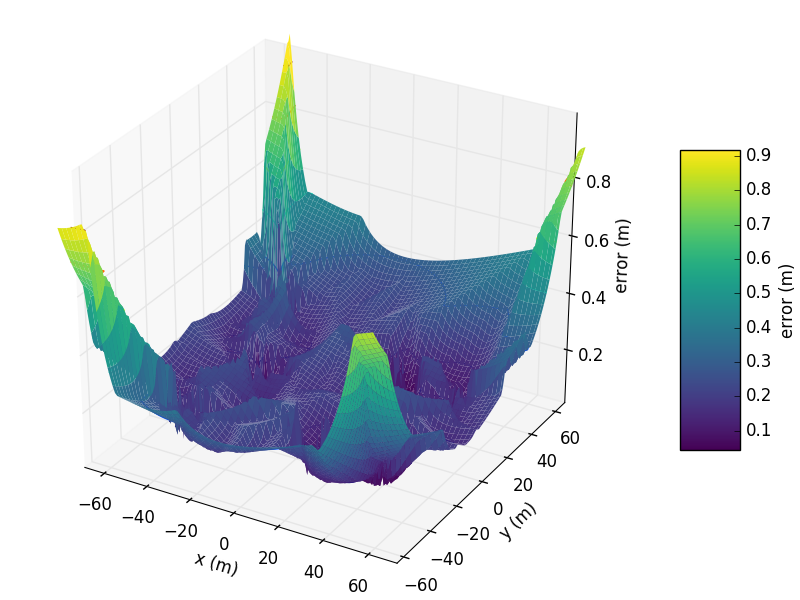
\includegraphics[width=0.5\textwidth]{heatmap}
 \caption{Heatmap d'erreur générée (le modèle d'erreur du capteur est ici arbitraire : 1cm + 2cm tous les 5m)}
 \label{fig:heatmap3D}
\end{figure}

%------------------------------------------------

\printbibliography
\end{document}
